\documentclass[a4paper,12pt]{article}
\usepackage[utf8]{inputenc}
\usepackage[margin=1in]{geometry}
\usepackage{graphicx}
\usepackage{array}
\usepackage{times}
\usepackage{listings}
\usepackage{color}
\usepackage{tikz}
\usetikzlibrary{shapes,arrows,positioning,calc}

\definecolor{dkgreen}{rgb}{0,0.6,0}
\definecolor{gray}{rgb}{0.5,0.5,0.5}
\definecolor{mauve}{rgb}{0.58,0,0.82}

\lstset{frame=tb,
  language=Java,
  aboveskip=3mm,
  belowskip=3mm,
  showstringspaces=false,
  columns=flexible,
  basicstyle={\small\ttfamily},
  numbers=none,
  numberstyle=\tiny\color{gray},
  keywordstyle=\color{blue},
  commentstyle=\color{dkgreen},
  stringstyle=\color{mauve},
  breaklines=true,
  breakatwhitespace=true,
  tabsize=3
}

\begin{document}

% --- Cover Page ---
\begin{center}
    \begin{figure}[h]
        \centering
        % \includegraphics[width=0.4\textwidth]{nmimslogo.png} 
        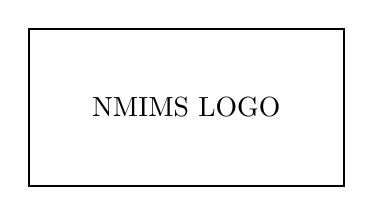
\begin{tikzpicture}
            \draw[thick] (0,0) rectangle (4,2) node[midway] {NMIMS LOGO};
        \end{tikzpicture}
        \caption*{Placeholder for nmimslogo.png}
    \end{figure}

    {\large \textbf{SVKM's NMIMS}} \\
    {\large Mukesh Patel School of Technology Management \& Engineering / \\ 
    School of Technology Management \& Engineering}

    \vspace{1cm}

    \renewcommand{\arraystretch}{1.5}
    \begin{tabular}{|l|l|}
        \hline
        \textbf{Year:-} II & \textbf{Program:-} B. Tech/MBA Tech \\ \hline
        \textbf{Semester:-} IV & \\ \hline
    \end{tabular}

    \vspace{1cm}

    {\Large \textbf{Subject:- Object-Oriented Programming through JAVA}} \\
    \vspace{0.5cm}
    {\large \textbf{Mini Project Title: Samarbhumi — War Never Ends}} \\
    {\large \textbf{Team Details: [INSERT TEAM NAMES]}}

    \vspace{1cm}

    \begin{tabular}{|l|p{3cm}|p{3cm}|p{3cm}|}
        \hline
        \textbf{Name} & & & \\ \hline
        \textbf{Roll No} & & & \\ \hline
        \textbf{SAP ID} & & & \\ \hline
    \end{tabular}

    \vspace{1.5cm}

    {\large Bachelor of Technology (Computer Science)} \\
    {Second Year, Semester IV} \\
    {Faculty: [NAME OF FACULTY]} \\
    {AY 2025-26}
\end{center}

\newpage

% --- Index Section ---
\section*{INDEX}
\addcontentsline{toc}{section}{INDEX}

\renewcommand{\arraystretch}{1.2}
\begin{tabular}{|c|l|c|}
    \hline
    \textbf{Sr. No.} & \textbf{Topic} & \textbf{Page No.} \\ \hline
    1 & Introduction & 3 \\ \hline
    2 & Requirement Analysis & 3 \\ \hline
    3 & Development Technologies & 4 \\ \hline
    4 & Modelling Classes & 5 \\ \hline
    5 & Progress Review (Week 10/11) & 9 \\ \hline
    6 & Implementation and Output & 10 \\ \hline
    7 & Observations and Learnings & 30 \\ \hline
    8 & Future Scope & 31 \\ \hline
    9 & Conclusion & 32 \\ \hline
\end{tabular}

\newpage

\section{Introduction}
\noindent \textbf{Samarbhumi} is a high-octane 2D arena shooter designed to showcase the capabilities of the Java programming language in the domain of real-time interactive systems. The project emphasizes low-latency networking, deterministic physics, and robust object-oriented architecture. Unlike modern games built on heavy engines, Samarbhumi is constructed from the ground up using native Java libraries, ensuring a lightweight yet powerful user experience.

\section{Requirement Analysis}

\subsection{Hardware Requirements}
\begin{itemize}
    \item \textbf{Processor:} Dual-core CPU clocking at 1.8 GHz or higher.
    \item \textbf{RAM:} Minimum 1 GB (2 GB recommended for online play).
    \item \textbf{Storage:} 50 MB of free disk space for game assets and logs.
    \item \textbf{Display:} $1280 \times 720$ resolution (standard) or higher.
\end{itemize}

\subsection{Software Requirements}
\begin{itemize}
    \item \textbf{Operating System:} Windows 10/11, macOS, or Linux.
    \item \textbf{Java Runtime:} Java Development Kit (JDK) 17 or higher.
    \item \textbf{Internet:} Stable connection for Multiplayer mode (Relay Server based).
\end{itemize}

\section{Development Technologies}

\subsection{Java 17+}
The core language utilized for all business logic, entity management, and networking. Java's robust type system and garbage collection allowed for rapid development of complex features.

\subsection{Swing \& AWT}
The graphical user interface (GUI) and rendering pipeline are built using \textit{javax.swing} and \textit{java.awt}. We utilized the \textit{BufferStrategy} class to implement triple-buffering, eliminating screen tearing and ensuring a smooth 60 FPS output.

\subsection{TCP/IP Sockets}
For the multiplayer component, \textit{java.net.Socket} was used to establish persistent connections between clients and a central relay server. This enables username-based lobby systems and real-time state synchronization.

\newpage

\section{Modelling Classes}

\subsection{Class Hierarchy Diagram}
\begin{center}
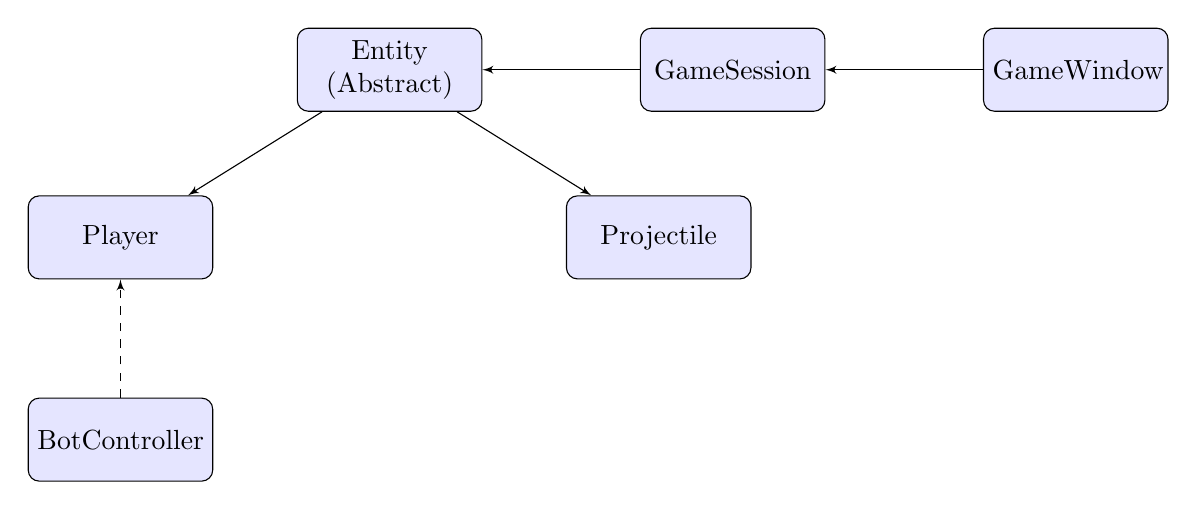
\begin{tikzpicture}[
    node distance=1.5cm,
    block/.style={rectangle, draw, fill=blue!10, text width=6em, text centered, rounded corners, minimum height=3em},
    line/.style={draw, -latex'}
]
    \node [block] (entity) {Entity (Abstract)};
    \node [block, below left=of entity] (player) {Player};
    \node [block, below right=of entity] (proj) {Projectile};
    \node [block, below=of player] (bot) {BotController};
    \node [block, right=2cm of entity] (session) {GameSession};
    \node [block, right=2cm of session] (window) {GameWindow};

    \path [line] (entity) -- (player);
    \path [line] (entity) -- (proj);
    \path [line] (session) -- (entity);
    \path [line] (window) -- (session);
    \path [line, dashed] (bot) -- (player);
\end{tikzpicture}
\end{center}

\subsection{Core Class Descriptions}
\begin{enumerate}
    \item \textbf{GameWindow:} The entry point and main controller. It manages the application state, renders the UI screens, and hosts the high-frequency game loop.
    \item \textbf{GameSession:} Orchestrates a single match. It maintains collections of players, projectiles, and pickups, and updates them at a fixed timestep.
    \item \textbf{NetworkSession:} A specialized subclass of GameSession that implements the Lockstep networking protocol, ensuring all clients stay synchronized.
    \item \textbf{NetManager:} Handles the low-level socket I/O, including handshake logic with the relay server and bit-masking input states.
\end{enumerate}

\section{Progress Review (Week 10/11)}
During these weeks, the focus shifted from single-player mechanics to the implementation of the online relay server. We successfully resolved the "Lobby Freeze" bug by moving network handshakes to asynchronous threads, ensuring the UI remained responsive during connection attempts.

\newpage

\section{Implementation and Output}

\subsection{Network Flow Diagram}
\begin{center}
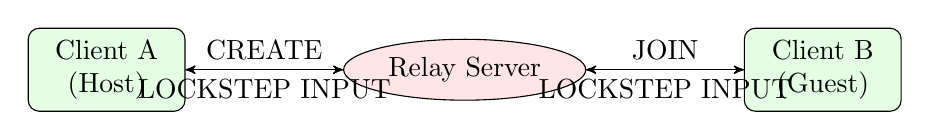
\begin{tikzpicture}[
    node distance=2cm,
    cloud/.style={draw, ellipse, fill=red!10, minimum height=2em},
    block/.style={rectangle, draw, fill=green!10, text width=5em, text centered, rounded corners, minimum height=3em},
    line/.style={draw, <->, >=stealth'}
]
    \node [block] (client1) {Client A (Host)};
    \node [cloud, right=of client1] (relay) {Relay Server};
    \node [block, right=of relay] (client2) {Client B (Guest)};

    \path [line] (client1) -- node[above] {CREATE} (relay);
    \path [line] (client2) -- node[above] {JOIN} (relay);
    \path [line] (relay) -- node[below, sloped] {LOCKSTEP INPUT} (client1);
    \path [line] (relay) -- node[below, sloped] {LOCKSTEP INPUT} (client2);
\end{tikzpicture}
\end{center}

\subsection{Code Snippet: Input Processing}
\begin{lstlisting}
public void update(float dt, InputState input) {
    if (isOnlineMatch) {
        // Deterministic Lockstep Check
        if (!NetManager.isFrameReady(currentFrame)) return;
        
        NetInput[] inputs = NetManager.consumeFrame(currentFrame);
        applyInputs(inputs);
        currentFrame++;
    }
}
\end{lstlisting}

\section{Observations and Learnings}
\begin{itemize}
    \item \textbf{Concurrency:} Managing shared state between the rendering thread and the network listener thread required careful use of \textit{ConcurrentHashMap} and volatile variables.
    \item \textbf{Synchronization:} Lockstep protocols are highly sensitive to latency; implementing a watchdog timer was essential for maintaining a viable user experience.
\end{itemize}

\section{Future Scope}
Future enhancements include the addition of a global leaderboard hosted on a relational database, more diverse character skills, and a procedural map generator to increase replayability.

\section{Conclusion}
Samarbhumi serves as a comprehensive demonstration of object-oriented principles applied to real-time systems. By building it in native Java, we achieved a high degree of control over performance and resource management.

\end{document}
